\section{Tracking and Vertexing}

Tracking, the procedure by which charged particle trajectories are reconstructed from a set of detector responses, and vertexing, the determination of the position along the beam line where particles from the two beams participated in a hard scattering, are interdependent at STAR. Both rely heavily on the TPC; in this analysis the TPC is the sole tracking detector, and TPC tracks are the primary source of information used by the vertex finder.  The tracker \cite{Rose:2003wx} and vertex finder \cite{vertex-finder-starnote} aspire to
%
\begin{itemize}
  \item find tracks based on a collection of hits from the tracking detectors,
  \item fit the hits associated to a track using a suitable track model,
  \item identify an event vertex and the subset of reconstructed tracks (called primary tracks) associated with that vertex,
  \item refit the primary tracks incorporating the event vertex, and
  \item calculate final state particle information for all reconstructed tracks.
\end{itemize}
%
The wide variety of collision types analyzed at STAR present a number of challenges for the tracking and vertexing software.  Head-on (central) collisions of gold atoms can produce 6000 or more charged particles in a single event, while high luminosity proton beams can generate up to $\sim$40 ``pile-up'' collisions in the TPC volume during the 40$\mu$s drift time required to read out a single triggered bunch crossing.

STAR employs a Kalman Filter approach to combine track finding and fitting into a single process.  The essence of the Kalman approach is that the current properties of a track segment are used to define the search space for the next hit to be added to the track, and when that next hit is added, the track properties are incrementally refined incorporating the new information.  The tracker starts by identifying a track seed, a short sequence of only a few hits containing the minimum amount of information needed to estimate the track's direction and curvature.  In principle these seeds could be constructed using hits from any region of the detector, but the most effective approach is to construct them using hits from the periphery of the TPC where the hit concentration is lowest.  The Kalman search proceeds to extrapolate this track seed inward to the next active layer of the detector, in this case a TPC pad row.  Matching hits on this layer are sought within a radius determined by the errors associated with the track extrapolation.  If no matching hit is found, the extrapolation moves on to the next layer.  If one or more hits are found, the filter calculates the increase in chi-square associated with the addition of each hit to the existing track segment and chooses the hit with the lowest incremental chi-square if it falls below a configurable threshold.  Once a hit is added, the track parameters are updated using the Kalman track model and the search continues on the next detector layer.  The search terminates when it reaches the innermost layer of the detector or when it passes some number of layers without finding any matching hits.  At the culmination of the search the track parameters calculated at the innermost hit offer the best description of the track; the other nodes can be considered under-constrained because they do not incorporate information from nodes that are closer to the origin.  An outward track refit is performed to rectify this situation.  The refit updates track parameters using the same methods as the initial search; the only difference from the search is that the hits are known in advance.

On occasion a track seed is identified deeper in the TPC; in these cases, an outward extrapolation of the track is warranted, and an outward search very similar to the inward one is performed.  Once this search is complete, the inner portion of the track is refit to incorporate the information from the new outer nodes.

The tracker continues the finding and fitting procedure with new track seeds until no more seeds are found.  The tracks identified at this stage of reconstruction do not incorporate any information about the position of the event vertex and are termed ``global tracks''.  Some global tracks are pileup tracks from events other than the one that triggered the detector, some correspond to the products of strange decays in the detector, and some really are ``primary tracks'' from particles produced in the hard scattering that fired the event trigger(s).  Determining which tracks belong in each category requires a precise knowledge of the position of the event vertex, and it turns out that the best calculation of the vertex position is one that relies on the global tracks themselves.

\subsection{Vertexing}

STAR uses different vertex finders optimized for the very different running conditions of heavy ion (MinuitVF) and proton-proton (PPV) collisions.  A detailed description of both can be found in STAR Note 488 \cite{vertex-finder-starnote}; the discussion here will focus on the Pile-Up Proof Vertexer (PPV), but many of the basic principles apply to both algorithms.  

One of PPV's major design goals is robustness in the face of high levels of pileup.  Pileup events usually occur in one of the $\sim$40 other bunch crossings that are read out along with the trigger bunch crossing by the TPC, although on rare occasions a single bunch crossing can contain multiple hard scatterings.  PPV does not try to guard against this in-time pileup, but it does work to suppress false event vertices from other bunch crossings.

PPV relies on a pre-calculated beam line constraint for the $x$ and $y$ position of each vertex.  The beam line constraint is determined by running the Minuit Vertex Finder on a subset of high-multiplicity events and fitting the resulting distribution of event vertices with a straight line.  PPV uses a subset of TPC tracks satisfying a series of quality cuts; these include a transverse momentum greater than 200 MeV, a distance of closest approach (DCA) to the beam line of less than 3 cm, and a requirement that the number of hits used to fit the track is at least 70\% of the maximum number of possible hits for the track's helix.  Each track is given an initial weight based on projection of its DCA in the $xy$ plane and the errors on the extrapolation to the beam line used to calculate that DCA.  The track's weight is increased if it is reconstructed from a minimum number of hits on both sides of the central membrane of the TPC or is matched to an energy deposit in the BEMC or EEMC, since tracks satisfying one or more of those conditions are very likely to have been produced in the bunch crossing that fired the trigger(s). A track with one of these positive weight adjustments is called a ``matched'' track. Conversely, if a track extrapolates to an active calorimeter tower without any energy deposit, or crosses the central membrane but has fewer than the minimum required number of hits on both sides of the membrane, the track's weight is reduced.  The total weight for the track is the product of the initial weight and each of these adjustments.

Vertices are identified by binning the $z$ axis with 1mm resolution and generating a histogram of all the track weights.  The peak of the histogram is the first vertex candidate; all tracks which extrapolate to within 3cm of this vertex position are grouped with the candidate and removed from further analysis.  PPV iterates this procedure until no more vertex candidates can be found. In the 2005 and 2006 runs PPV required at least two ``matched'' tracks in order to save a vertex; that requirement has been relaxed in recent years to improve the vertex finding efficiency for forward triggers, which have event topologies that make it unlikely to find two tracks in an event satisfying the matching conditions.  PPV saves multiple vertices for each event, ordered by rank; in 2005 and 2006, the rank is simply the cumulative weight of all the tracks in the vertex.  The vertex finding efficiency is highly trigger-dependent; Table \ref{tbl:vertex-finding-efficiencies} lists the fraction of events with at least one primary vertex in each of the triggers used for this analysis.

\begin{table}
  \begin{center}
    \begin{tabular}{cc|ccc}
      \hline
      year & trigger ID & total events & events with vertex & efficiency\\
      \hline
      \hline
      2005 & MB (96011) & 0 & 0 & 0\\
      \hline
      2005 & BJP1 (96221) & 0 & 0 & 0\\
      \hline
      2005 & BJP2 (96233) & 0 & 0 & 0\\
      \hline
      2006 & MB (117001) & 0 & 0 & 0\\
      \hline
      2006 & BJP1 (13722[1-2]) & 0 & 0 & 0\\
      \hline
    \end{tabular}
  \end{center}
  \caption{Vertex Finding Efficiencies}
  \label{tbl:vertex-finding-efficiencies}
\end{table}

Once the vertices have been identified, the tracker adds the vertex position as an additional hit to every track associated with that vertex and refits those tracks.  The STAR software framework saves this collection of ``primary'' tracks as well as the original ``global'' tracks.  In this analysis primary tracks are used exclusively; the global tracks associated with those primaries are only analyzed to apply a more stringent cut on the DCA to the primary vertex position obtained from the original track extrapolation.

\begin{figure}
  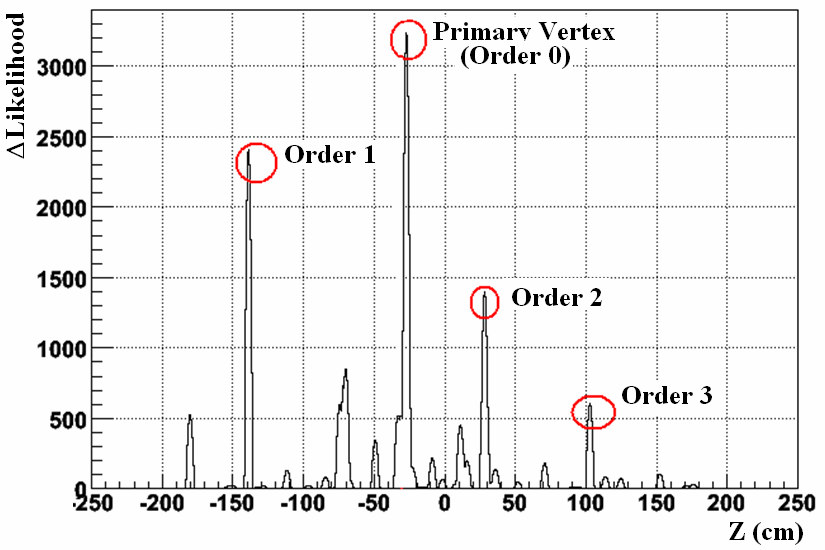
\includegraphics[width=1.0\textwidth]{figures/ppv-candidate-distribution}
  \caption{Example vertex candidate distribution generated by PPV \cite{vertex-finder-starnote}. An ordered list of vertices is extracted from the peaks of this distribution, with the requirement that each vertex contains at least two tracks satisfying the matching conditions.}
  \label{fig:ppv-candidate-distribution}
\end{figure}
